% Author attachment: pasted-text-2026-10-10_23-16-35-189.md

% Wording and values preserved; only LaTeX escaping and reference integration.

\section{Ablations}

% Queue Figure 5 early so it can occupy the top-left column on page 7.
\begingroup
\let\ablationfigure\figure
\renewcommand{\figure}[1][]{\ablationfigure[!t]}
\begin{figure}[!htbp]
\centering
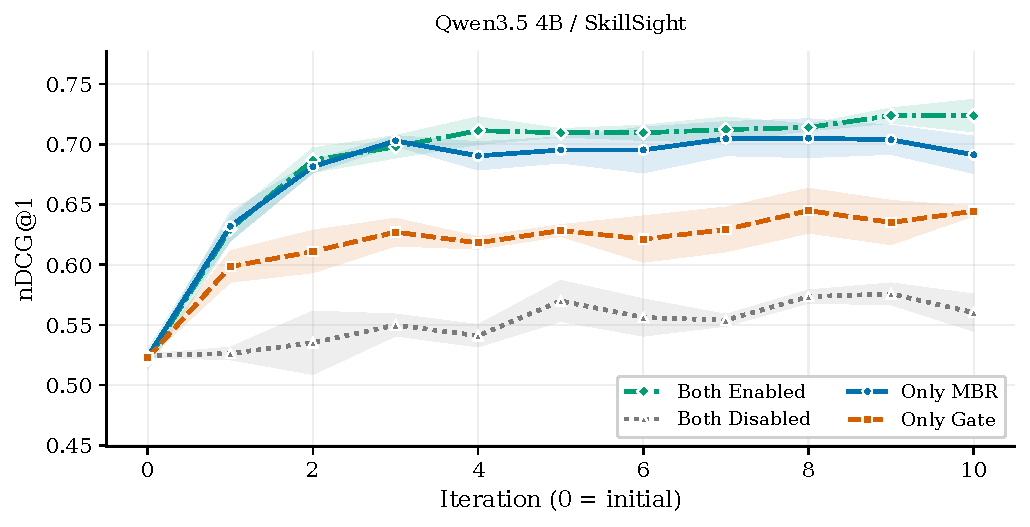
\includegraphics[width=\linewidth]{figs/mbr_replay_test_ndcg@1_std/preview.pdf}
\caption[Replay and validation-gate ablation: test nDCG@1]{\input{figs/mbr_replay_test_ndcg@1_std/description.text}}
\label{fig:mbr_replay_test_ndcg@1_std}
\end{figure}

\endgroup

\subsection{Impact of MBR based on Replay and Held-out Validation Gate}

Figure~\ref{fig:mbr_replay_test_ndcg@1_std} shows MBR with bounded replay alone achieved higher final performance on test dataset than the held-out validation gate alone: F1 increased from 0.495 to 0.594 and nDCG@1 from 0.644 to 0.691, relative improvements of 20.0\% and 7.3\%, respectively. Combining MBR with the held-out gate further improved final performance on unseen test tasks, increasing F1 by 3.28\% and nDCG@1 by 4.71\% to 0.724 compared with MBR alone. Relative to each configuration's own initialization, disabling both only increases F1 and nDCG@1 by 21.0\% and 6.8\% which is much lower than the 100.9\% and 38.8\% increase when both are enabled. This supports empirical update selection without implying that unchecked updates invariably worsen performance. With both components enabled, diminishing returns appeared around iteration 5, by which point 96.5\% of the final F1 gain and 93.0\% of the final net nDCG@1 gain had accrued. Later iterations added only 0.011 F1 and 0.014 nDCG@1, indicating an approximate plateau. This suggest diminishing opportunities for useful predicate refinement on the plateau: early iterations correct broad, frequent routing errors, while later iterations encounter harder or less common cases.

\subsection{Performance and Token Usage Tradeoff of MBR Replay and Held-out Gate}

Figure~\ref{fig:performance_token_usage} demonstrates that combining replay and the gate provides the strongest final routing performance, while MBR alone reduces token usage by 10.8\% at the cost of a 7.7\% relative decrease in nDCG@1 compared with using both. Across configurations with and without the gate, replay improves final routing performance by 15.4\% to 23.7\% at the cost of a  40.6\% to 52.9\% increase in token usage.

\subsection{Skill Routing Performance across LLM Backbones}

As shown in Figure~\ref{fig:routing_performance_across_llms_init}, the cold-start nDCG@1 scores of Qwen3.5 4B, Qwen3.8 27B, and GPT-OSS 120B are 0.520, 0.635, and 0.686, respectively. RouterBSI optimization increases these scores to 0.742, 0.802, and 0.745, corresponding to relative improvements of 42.7\%, 26.3\%, and 8.6\%. Although the relative gain decreases with model size, the final scores are not monotonic: Qwen3.8 27B achieves the highest nDCG@1 among these backbones. The optimized RouterBSI with Qwen3.5 4B approaches GPT-OSS 120B performance, reaching 99.6\% of the GPT-OSS 120B performance. Overall, these results demonstrate that RouterBSI can significantly improve the routing performance of predicates across LLMs. They also suggest that predicates reach a plateau that cannot be overcomed with more capable LLMs, where it's difficult for the predicate to be narrow enough to be false for irrelevant tasks but broad enough to be true for all relevant tasks

\begin{figure}[!htbp]
\centering
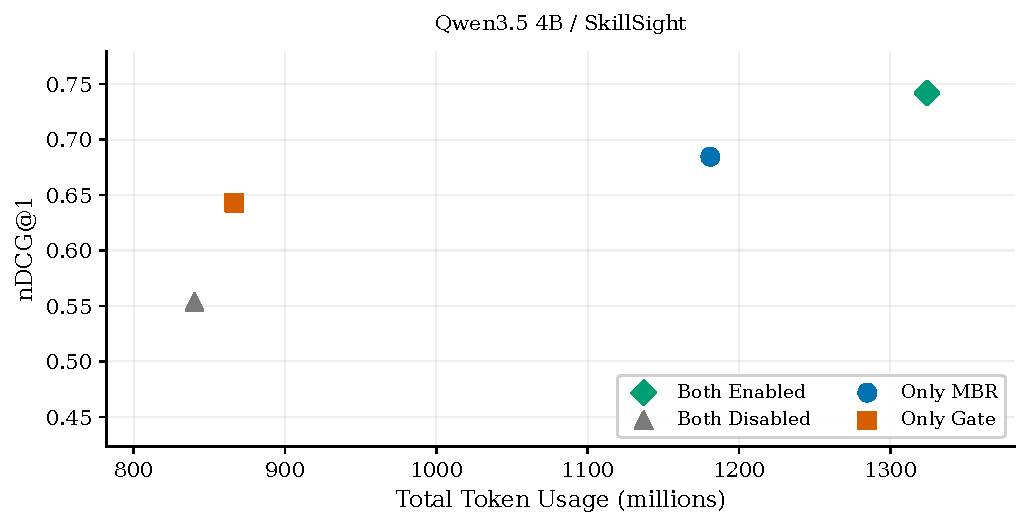
\includegraphics[width=\linewidth]{figs/performance_token_usage/preview.pdf}
\caption{Impact of MBR replay and held-out validation gate on routing performance (nDCG@1) and token usage. Both enabled gives the strongest performance. MBR alone uses fewer tokens at a performance cost.}
\label{fig:performance_token_usage}
\end{figure}


% Defer Figure 7 after Figure 6 is numbered, while prose continues to flow.
\afterpage{%
\begingroup
\let\backbonepagefigure\figure
\renewcommand{\figure}[1][]{\backbonepagefigure[!ht]}
\begin{figure}[!htbp]
\centering
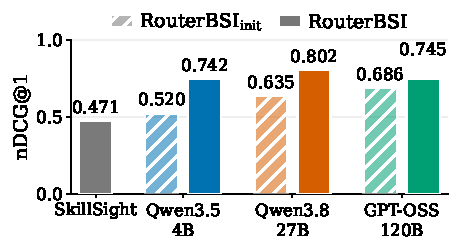
\includegraphics[width=\linewidth]{figs/routing_performance_across_llms_init/preview.pdf}
\caption[Routing performance by language-model backbone]{\input{figs/routing_performance_across_llms_init/description.text}}
\label{fig:routing_performance_across_llms_init}
\end{figure}

\endgroup
}

